\acresetall
\chapter{Evaluation}\label{ch:chapter4}

In this chapter, we present the evaluation of \emph{Ferify}. The first section includes the validation tests we performed. These tests represent the cases \emph{Ferify} can be employed. The next section covers the performance overhead tests we performed to evaluate the degree our solution impacts overall system usability.

\section{Validation}\label{sec:validation}

\par To assess that \emph{Ferify} works as intended, we assume two basic scenarios. The first is that of an authorized remotely connected user, who should be able to work as before. We want usability at the user level to remain unchanged. The second scenario is that of a hacked user account. The attacker has managed to exploit a vulnerability of the guest \ac{OS} and has remote access to the target \ac{VM}. In this case we assume even the worst case scenario that the attacker has gained \emph{root} privileges. We want to assess whether the files we protect with \emph{Ferify} are secure and cannot be accessed except from those we have allowed in the \acp{SACL}.

\par To emulate the actions of an attacker, we performed specific commands on the guest \ac{VM} in order to observe the behavior of the system and whether it conforms to the expectations. The commands reflect the cases that \emph{Ferify} can be applied and correspond to the most basic commands one can issue. All higher level programs and attacks eventually resort to the execution of these system calls. To do that we created an environmental setup to assess all the test cases. 

\par The configuration includes two users, \emph{alice} and \emph{bob}, both in the sudoers group, but \emph{bob} not legitimately, but through malicious actions. The intent is to check the detection of the illegal escalation of \emph{bob}'s account to \emph{root} and the effect it has.

\par Additionally we created a group that includes both users, with the intention to assess the per group policy enforcement to file access. 

\par Finally we will try, as \emph{root}, to access files that are being protected from root. These files include the \emph{/etc/shadow} file and the \emph{/etc/pam.d/su}, which are included in the \acp{SACL} to protect our initial \ac{VM} configuration.

\par These cases by themselves cover the basic set of actions that \emph{Ferify} was initially designed to monitor. Any combination of them is handled separately from the underlying \ac{OS}, reducing our problem to these elementary cases, making it easier to monitor and handle.

\par First we will test if an illegal \emph{root} escalation is possible and then we will test the file operations, which include \emph{create, open, read, write, copy, move, delete, and link}.

\subsection{Root escalation}

\par One of the first actions of an attacker or malicious program is to try to escalate its privileges to that of the root account. One of those techniques is to add the compromised user to the \emph{sudoers} group. To avoid such an exploitation, every time a trap gets caught by the hypervisor we check whether the user executing a \emph{sudo} command is actually allowed to, according to the initial administrative setup of \emph{Ferify} for the specific \ac{VM}. If the user is a legitimate \emph{sudoer} the flow of our plugin continues normally to check the validity of the file operation against the \acp{SACL}. On the other hand, if the user is not supposed to have \emph{sudo} privileges, the system calls, trapped by \emph{Ferify}, that get invoked get canceled, denying the ability to perform any \emph{sudo} command. Figure \ref{fig:sudo_deny} shows the result of trying to execute a \emph{sudo} command that gets denied, while at the same time we get notified on the hypervisor of the event as shown in fig. \ref{fig:sudo_deny_not}.

\begin{figure}[ht]
	\centering
	\footnotesize{\fontfamily{qcr}\selectfont 
		\begin{lstlisting}
bob@aHVM-domU:~$ sudo ls
sudo: unable to open /etc/sudoers: Bad address
sudo: no valid sudoers sources found, quitting
sudo: unable to initialize policy plugin
bob@aHVM-domU:~$
		\end{lstlisting}}
	\caption{Denying \emph{sudo}}
	\label{fig:sudo_deny}
\end{figure}

\begin{figure}[ht]
	\centering
	\footnotesize{\fontfamily{qcr}\selectfont 
		\begin{lstlisting}
Warning: Process root identity corruption detected in task 
	1377! Is 0 and should be 1002. 
	Invalidating syscall.
[SYSCALL:   2] CR3:0x1afec000  , RDI: 0x7f2178a931f7 ,sudo 
	PID:1377 [0:1002] wants 0 access to file: 
	/etc/sudoers (mode:0)
		\end{lstlisting}}
	\caption{Denying \emph{sudo} notification on the hypervisor}
	\label{fig:sudo_deny_not}
\end{figure}

\par In the same manner the result of trying to change a users password shows in fig. \ref{fig:passwd_deny}

\begin{figure}[ht]
	\centering
	\footnotesize{\fontfamily{qcr}\selectfont 
		\begin{lstlisting}
bob@aHVM-domU:~$ passwd alice
Enter new UNIX password:
Retype new UNIX password:
passwd: Authentication token manipulation error
passwd: password unchanged
bob@aHVM-domU:~$
		\end{lstlisting}}
	\caption{Denying password change from \emph{root} account}
	\label{fig:passwd_deny}
\end{figure}


\par Having solved the issue of malicious root access, we then need to validate the expected behavior for file access, whether requested from the \emph{root} user or not.

\subsection{Authorized user operation}

\par A very important aspect of a security solution is the impact on usability for the normal user. The implementation of a secure system that remains fully usable is a challenge. In this test we evaluate whether an authorized user can normally access and work on his files. 

\subsection{Attacker operation}



%\par One of the issues in the Linux file access permission system is that if a file belongs to a group, all users in that group can access the file, given the \ac{ACL} allows it. There are cases when a user wants to protect a file from being accessed but cannot, because other users belong to the same group, or multiple groups can access the file. 

%\par For this setup we created a third user \emph{jim}, who belongs only to the group \emph{alice} and a file owned by user and group \emph{alice}. There are two configurations available in the case of group access. User \emph{bob} belongs also to group \emph{alice} as a secondary group. Therefore, in this case all three users \emph{alice, bob, jim} have access to the file. By adding an entry to the \ac{SACL} for the file, with permissions \emph{rw-r-----} or \emph{640}, we effectively can deny access to anyone who belongs to group \emph{alice} as a secondary group, in this case user \emph{bob}. The results of the read operation for \emph{bob} and \emph{jim} show in fig. \ref{fig:sec_group_deny}

%\begin{figure}[ht]
%	\centering
%	\footnotesize{\fontfamily{qcr}\selectfont 
%		\begin{lstlisting}
%bob@HVM-domU:~$ more /home/alice/file_in_group_alice
%more: cannot open /home/alice/file_in_group_alice: 
%	Bad address
%
%jim@HVM-domU:~$ more /home/alice/file_in_group_alice
%Bob should not read this...
%		\end{lstlisting}}
%	\caption{Denying access from secondary group users}
%	\label{fig:sec_group_deny}
%\end{figure}
%
%\par By changing the permissions of the file to \emph{rw-------} or \emph{600} we deny access to everyone except for the actual owner of the file, in this case \emph{alice}. The same setup can be accomplished directly by changing the permissions of the file, but by using this solution, we can confuse the attackers, since it seems that they should have access as a group user. Now, not even user \emph{jim} has access to the file, although he should, as shown in fig. \ref{fig:group_deny}
%
%\begin{figure}[ht]
%	\centering
%	\footnotesize{\fontfamily{qcr}\selectfont 
%		\begin{lstlisting}
%jim@HVM-domU:~$ more /home/alice/file_in_group_alice
%more: cannot open /home/alice/file_in_group_alice: 
%	Bad address
%		\end{lstlisting}}
%	\caption{Denying access from group users}
%	\label{fig:group_deny}
%\end{figure}

\subsection{Root access}

\par One of the biggest problems in computer security is the fact that the \emph{root} user or the \emph{administrator} of the system has access to all the files of the system. That is the reason most attacks try to result in escalation of privileges to an administrative account. Although a system administrator should have access to all \ac{OS} files for management issues, some user files with critical information are also visible or editable. With \emph{Ferify} we can change the administrator's file access permissions to those we need to enforce, whether no access at all, read-only, or write-only.

\subsection{Malware Protection}

\subsection{Append-only mode}

\par Although we could not enforce partial write permissions to a file, due to the \ac{OS} limitations. A file can be opened as a whole, given the permissions the user requests. What \emph{Ferify} is capable of doing is to enforce a write-only access policy to files. This way, if attackers want to cover their tracks, they are not able to open a file in read-write mode, to select and delete the log entries that reveal their presence. They will have to blindly delete entries, or empty the entire log, action that should be noticed by the system administrator. We believe that this policy can be proven a substantial hindrance to malicious actors that try to coven their tracks in the system.

\section{Performance overhead}\label{sec:performance}

In this section we present the performance overhead we observed on the guest \ac{OS} when running \emph{Ferify}. We performed time execution measurements in four stages. 

\par To have a baseline for comparison, we created a script which accesses a series of files, in order to trigger \emph{Ferify}, when it is running. Initially we timed the execution of the script over a number of iterations to extract an average time that we will use as a reference. 

\subsection{Hypervisor - \ac{VM} switch}

\par One of the most intense operations in virtualization is the switch between the hypervisor and the \ac{VM}, as mentioned in subsection \ref{sub:invm}. \ac{CPU} virtualization extensions improve with every new model release, but this switch is still significant. To measure this overhead in performance, we ran \emph{Ferify} with empty \acp{SACL}. This way \emph{Ferify} traps the appropriate system calls and performs the switch between the \ac{VM} and the hypervisor. Because the \acp{SACL} are empty, there is insignificant computation performed while on the hypervisor, switching almost immediately back to the \ac{VM}. 


\subsection{Small \ac{SACL} performance overhead}

\par The information for the files stored in the \acp{SACL} is stored in an array of linked lists. The index of the array is the length of the pathname. Then all pathnames of the same length are stored in the same linked list. When only a few files are protected, these linked lists are very short, if not of size one or two. This makes the lookup process fast and easy. 

\subsection{Large \ac{SACL} performance overhead}

\par Adding more files to the \acp{SACL} may add a more substantial overhead. As shown in \ref{fig:pathname_length}, there is a significant amount of pathnames with lengths between 10 and 130. Having so many elements in a linked list introduces increased time in searching for a record. To assess the performance overhead we repeated the previous test, but this time after adding more than 1000 files in the \acp{SACL}. Writing \acp{ACL} for thousands of files is extremely time-consuming and error-prone. To automate this procedure we created a standalone script that pauses the guest \ac{VM}, mounts its filesystem to the hypervisor and starting from a specified mount-point, it returns the required information. 

\par After having generated a \ac{SACL} that corresponds to the current guest \ac{OS} filesystem permissions, the administrator can easily modify the permissions to reflect the desired policy to be enforced. 

\begin{figure}[ht]
	\centering
	%\begin{tikzpicture}
\begin{axis}[
title={Pathname length distribution of sample \ac{OS}},
xlabel={Pathname length},
ylabel={Count (thousands)},
xmin=0, xmax=600,
ymin=0, ymax=27000,
xtick={0,100,200,300,400,500,600},
ytick={0, 5000, 10000, 15000, 20000, 25000},
ymajorgrids=true,
xmajorgrids=true,
grid style=dashed,
]

\addplot[very thick, blue, smooth] table [
col sep=comma,
x = Length,
y = Count,
] {figs/graph1.csv};

\end{axis}
\end{tikzpicture}
	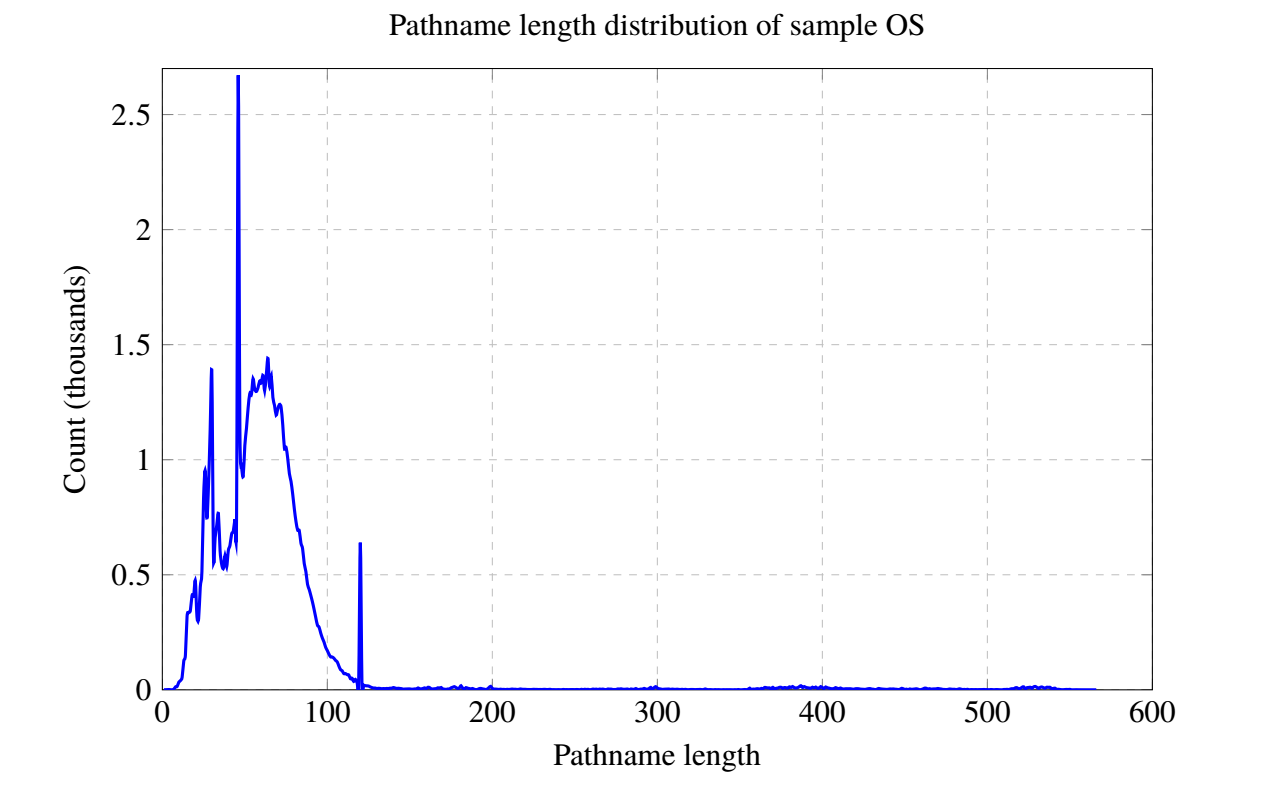
\includegraphics[scale=0.45]{images/graph1.png}
	\caption{Pathname length count}
	\label{fig:pathname_length}
\end{figure}


\subsection{Full \ac{OS} \ac{SACL} performance overhead}

\par Finally, we wanted to evaluate whether \emph{Ferify} can be used on the whole filesystem of a guest \ac{OS}. To do that we just created a \ac{SACL} that was generated by the aforementioned script when providing as mount-point the root folder of the guest \ac{OS}. Since the vast majority of the files is in the same range of length, we expect significant delays in our script execution.




